\documentclass[12pt]{article}
\usepackage{tikz}
\usetikzlibrary{arrows}
\begin{document}
\begin{figure}
\begin{center}
% con l'ambiente tikz in latek si possono rappresentare disegni e schemi
% di vario tipo.
\begin{tikzpicture}

% con node
% qui vado a definire i disegni in questione. In ordine di apparizione:
% [draw,circle] --> disegna un cerchio
% (s1) at (0,0) --> nome dell'oggetto e dove viene posizionato
% {A} --> contenuto del'oggetto in questione.
\node[draw,circle] (s1) at (0,0) {A};
\node[draw,circle] (s2) at (-1.6,-2) {B};
\node[draw,circle] (s3) at (1.6,-2) {C};
\node[draw,circle] (s4) at (-4,-3) {D};
\node (s5) at (4,-3) {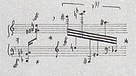
\includegraphics[width=2cm]{serenata.jpg}};

% in path vado a definire i collegamenti, ad esempio:
% (s2) edge[->, double distance=1pt, >=latex', bend left=40] (s1)
% definisce che l'oggetto (s2) punterà con edge all'oggetto (s1)
% con i parametri [->, double distance=1pt, >=latex', bend left=40]
\path
    (s2) edge[->, double distance=1pt, >=latex', bend left=40] (s1)
    (s3) edge[->, double distance=1pt, >=latex', bend right=40] (s1)
    (s3) edge[->, double distance=1pt, >=latex', bend left=60] (s2)
    (s2) edge[<->, double distance=1pt, >=latex'] (s4)
    (s3) edge[<->, double distance=1pt, >=latex'] (s5);

% dopo di chè, chiudo tikz.
\end{tikzpicture}

\end{center}
% commento del tutto:
\caption{Prove di stato a 5 parti}
% il commento punta a:
\label{fig1}

% chiudo figure
\end{figure}

% concludo
\end{document}